% !TEX root = prace.tex
\chapter{Učení parametrů}
\label{ch:ep}

Představená metoda LBP v~minulé kapitole funguje pro modely, kde máme nastavené parametry faktorů.
V~této kapitole si představíme grafický model pro diskrétní proměnné, u~kterého jsou i parametry faktorů proměnné a je možné pro ně použít Bayesovský přístup.
Díky tomu bude možné nalézt aposteriorní distribuci pro tyto parametry a naučit je podle dat.

Inferenci v~tomto upraveném modelu už není možné dělat pomocí LBP a~budeme muset použít algoritmus Expectation Propagation.

\section{Grafický model}

Model se skládá z~faktorů a proměnných.
Nechť máme vybraný faktor $f_\beta$, spojený s~několika proměnnými
$\vec{x} = (x_0, x_1, \dots, x_{N_x})$
a množinami parametrů
$\vec{\Theta} = (\vec{\theta}_1, \dots, \vec{\theta}_{N_\theta})$.
Tento faktor reprezentuje podmíněnou pravděpodobnost:
$$f_\beta(\vec{x}, \Theta) = p(x_0 | x_1, \dots, x_{N_x}; \Theta).$$

Rodičovské proměnné $x_1, \dots, x_{N_x}$ označujeme jako $\vec{x^\prime}$.
Vektor $\vec{x^\prime}$ určuje, jaká množina parametrů bude použita.
Protože množiny parametrů jsou číslovány $1, \dots, N_\theta$ a rodičovské
proměnné $1, \dots, N_x$, musí být pro vybrání správné množiny parametrů
použito mapování $\rho(\vec{x^\prime})$.
Faktor pak může být zapsán zkráceně:
$$f_\beta(\vec{x}, \Theta) = p(x_0 | x_1, \dots, x_{N_x}; \Theta) =
\theta_{\rho(x^\prime), x_0}$$

Příklad faktoru $f_\beta$ je na obrázku~\ref{ex:factor}, pro ilustraci pouze s~třemi parametry a čtyřmi proměnnými.
Správně by měl faktor mít tolik parametrů, kolik je možných přiřazení pro rodičovské proměnné.

\begin{figure}[h]
\begin{center}
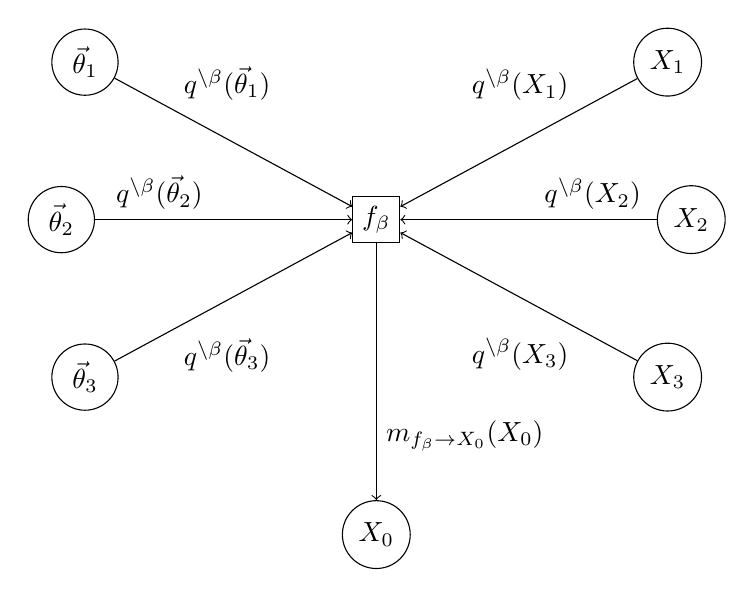
\begin{tikzpicture}[->, main/.style={circle, draw}, factor/.style={draw}]
    
\node[main] at (-3.7, 2)    (t1) {$\vec\theta_1$};
\node[main] at (-4, 0)      (t2) {$\vec\theta_2$};
\node[main] at (-3.7, -2)   (t3) {$\vec\theta_3$};
\node[factor] at (0, 0)     (f)  {$f_\beta$};
\node[main] at (3.7, 2)     (x1) {$X_1$};
\node[main] at (4, 0)       (x2) {$X_2$};
\node[main] at (3.7, -2)    (x3) {$X_3$};
\node[main] at (0, -4)      (x0) {$X_0$};

\path
	(t1) edge [above right, near start] node {$q^{\backslash \beta}(\vec\theta_1)$} (f)
	(t2) edge [above, near start] node {$q^{\backslash \beta}(\vec\theta_2)$} (f)
	(t3) edge [below right, near start] node {$q^{\backslash \beta}(\vec\theta_3)$} (f)
	(x1) edge [above left, near start] node {$q^{\backslash \beta}(X_1)$} (f)
	(x2) edge [above, near start] node {$q^{\backslash \beta}(X_2)$} (f)
	(x3) edge [below left, near start] node {$q^{\backslash \beta}(X_3)$} (f)
	(f) edge [right, near end] node {$m_{f_\beta \rightarrow X_0}(X_0)$} (x0);


\end{tikzpicture}
\end{center}
\caption{Vybraný faktor $f_\beta$ pro aktualizaci při učení parametrů.}
\label{ex:factor}
\end{figure}

\section{Výpočet marginálních pravděpodobností}

Pro výpočet sdružené pravděpodobnosti používáme plně faktorizovanou distribuci.
Pro každou proměnnou (množinu parametrů) je její marginální pravděpodobnost
rovna součinu zpráv ze sousedních faktorů.
Pro daný faktor $f_\beta$ je neúplná distribuce $q^{\backslash \beta}(x_i)$, popř.
$q^{\backslash \beta}(\vec{\theta}_i)$, rovna součinu zpráv ze všech ostatních faktorů do $x_i$, popř $\vec\theta_i$.
Aproximovaná marginální pravděpodobnost proměnné (množiny parametrů) je pak součinem neúplné
distribuce a zprávy z~faktoru:
$$q(x_i) = q^{\backslash \beta}(x_i) m_{f_\beta \rightarrow x_i}(x_i), 
\quad \quad
q(\vec{\theta}_i) = q^{\backslash \beta}(\vec{\theta}_i) m_{f_\beta \rightarrow \theta}(\vec{\theta}_i)$$

Tyto neúplné distribuce jsou právě zprávy z~proměnné, popř. množiny parametrů, do faktoru:

$$m_{x_i \rightarrow f_\beta} = q^{\backslash \beta}(x_i), 
\quad \quad
m_{\vec\theta_i \rightarrow f_\beta} = q^{\backslash \beta}(\vec\theta_i).$$

\subsection{Marginální pravděpodobnost proměnných}

Pokud chceme aktualizovat hodnotu naší aproximace marginální pravděpodobnosti,
je třeba minimalizovat její vzdálenost od skutečné marginální
pravděpodobnosti, ve tvaru
\begin{align}
p^*(\tilde{x}_j) &=
\sum_{\vec{x} \backslash x_j} \,
	\int_{\vec{\Theta}} \,
    		\prod_i \,
			q^{\backslash \beta}(x_i) \,
		\prod_l \,
			q^{\backslash \beta}(\vec{\theta}_l) \;
		f_\beta(\vec{x};\,
    		  \vec{\Theta})
\label{eq:1} 
\\
&=
\sum_{\vec{x} \backslash x_j} \,
	\prod_i \,
		q^{\backslash \beta}(x_i) \,
    \int_{\vec{\theta_{\rho(\vec{x^\prime})}}} \,
	    q^{\backslash \beta}(\vec{\theta}_{\rho(\vec{x^\prime})})\;
    \theta_{\rho(\vec{x^\prime}), x_0} \label{eq:2} 
\\
&= 
\sum_{\vec{x} \backslash x_j} \,
	\prod_i \,
		q^{\backslash \beta}(x_i)\;
    		\mathbb{E}_{q^{\backslash \beta}} 
			(\theta_{\rho(\vec{x^\prime}), x_0}).
\label{eq:3}
\end{align}

Rovnost~(\ref{eq:1}) vychází z~definice výpočtu marginální pravděpodobnosti ze
sdružené pravděpodobnosti.
V~(\ref{eq:2}) byla použita definice faktoru, z~integrálu byly vytknuty členy neobsahující $\Theta$ a nakonec bylo využito toho, že pro
množiny parametrů, které nejsou spojeny s~faktorem $f_\beta$, je jejich neúplná
distribuce rovna marginální distribuci a tedy $\int_{\theta_i} q(\theta_i) =
1$. V~(\ref{eq:3}) byla použita definice očekávané hodnoty.

Marginální pravděpodobnost proměnné $x_i$ tedy je
\begin{equation}
p^*(x_i) =
\sum_{\vec{x} \backslash x_j} \;
	\prod_i \;
		q^{\backslash \beta}(x_i)\;
    		\mathbb{E}_{q^{\backslash \beta}} 
			(\theta_{\rho(\vec{x^\prime}), x_0}).
\end{equation}

Tady docházíme k~výsledku, který je velmi podobný výpočtu marginální
pravděpodobnosti v~Loopy Belief Propagation algoritmu.

Zprávu z~faktoru $f_\beta$ do vrcholu $x_j$ pak získáme vydělením zprávy z~$x_j$ do $f_\beta$ z~marginální pravděpodobnosti,

\begin{equation}
m_{f_\beta \rightarrow x_j}(x_j) =
    \sum_{\vec{x} \backslash x_j} \;
        \prod_{i \ne j}\;
            q^{\backslash \beta}(x_i)\;
            \mathbb{E}_{q^{\backslash \beta}}
                (\theta_{\rho(\vec{x^\prime}), x_0}).
\label{eq:msgfromftox}
\end{equation}

\subsection{Marginální pravděpodobnost parametrů}

Pro množiny parametrů se jejich marginální pravděpodobnost spočítá podobně jako
pro proměnné:
\begin{align}
p^*(\tilde{\vec{\theta}}_j) & = 
    \sum_{\vec{x}} \; 
    \int_{\vec{\Theta}: \vec{\theta}_j = \tilde{\vec{\theta}}_j} \;
         \prod_i \;
             q^{\backslash \beta}(x_i) \;
         \prod_l \;
    q^{\backslash \beta}(\vec{\theta}_l) \;
    f_\beta(\vec{x}; \vec{\Theta}) \label{eq:ep:theta_1}
\\
& = 
    \sum_{l \ne j} \;
        \sum_{\vec{x}: \rho(\vec{x^\prime}) = l} \;
            \prod_i \;
                q^{\backslash \beta}(x_i) \,
                \int_{\vec{\Theta}: \vec{\theta}_j = \tilde{\vec{\theta}}_j} \;
                    \prod_k \;
                        q^{\backslash \beta}(\vec{\theta}_k) \;
                        \theta_{l, x_0}\; + \label{eq:ep:theta_2}
\\
& + 
    \sum_{\vec{x}: \rho(\vec{x^\prime}) = j} \;
        \prod_i \;
            q^{\backslash \beta}(x_i) \;
            \int_{\vec{\Theta}: \vec{\theta}_j = \tilde{\vec{\theta}}_j} \;
                \prod_k \;
                    q^{\backslash \beta}(\vec{\theta}_k) \; 
                    \tilde{\theta}_{j, x_0}
\nonumber
\\
& = 
    \left[ \;
        \sum_{l \ne j} \;
            \sum_{\vec{x}: \rho(\vec{x^\prime}) = l} \;
                \prod_i \;
                    q^{\backslash \beta}(x_i) \;
                    \mathbb{E}_{q^{\backslash \beta}(\vec{\theta}_l)} (\theta_{l, x_0}) \;
    \right] \;
    q^{\backslash \beta}(\tilde{\vec{\theta}}_j) \; + \label{eq:ep:theta_3}
\\
& + 
    \sum_{\vec{x}: \rho(\vec{x^\prime}) = j} \;
        \prod_i \;
            q^{\backslash \beta}(x_i) \;
            \tilde{\theta}_{j,x_0} \;
            q^{\backslash \beta}(\tilde{\vec{\theta}}_j) \;
\label{eq:ep:theta_4}
\nonumber
\\
& = w_0 \; q^{\backslash \beta}(\tilde{\vec{\theta}}_j) \, + \, \sum_k \; w_k \;
    \tilde{\theta}_{j,k} \; q^{\backslash \beta}(\tilde{\vec{\theta}}_j),
\end{align}

kde

\begin{align}
w_0 &=
	\sum_{l \ne j} \;
		\sum_{\vec{x}: \rho(\vec{x^\prime}) = l} \;
			\prod_i \;
 				q^{\backslash \beta}(x_i) \;
				\mathbb{E}_{q^{\backslash \beta}(\vec{\theta}_l)} (
					\theta_{l,
					x_0}) 
\\
w_k &=
	\sum_{\vec{x}: \rho(\vec{x^\prime}) = j, x_0 = k} \; 
		\prod_i \;
			q^{\backslash \beta}(x_i)		
\end{align}

Opět vycházíme z~výpočtu marginální pravděpodobnosti podle definice.
V~rovnici \eqref{eq:ep:theta_2} jsme rozdělili sumu přes
$\vec{x}$ na ty, pro které se ve faktoru použije množina parametrů
$\tilde{\vec{\theta}}_j$, a na ty ostatní. Také jsme z~integrálu vytknuli součin
neúplných distribucí pro proměnné. V~dalším kroku \eqref{eq:ep:theta_3} jsme opět
použili toho, že integrál přes $\vec{\Theta}$ je ve skutečnosti několik
integrálů přes jednotlivé množiny parametrů. Díky tomu je můžeme vložit mezi členy produktu neúplných distribucí pro množiny parametrů. Ve výsledku
získáme $q^{\backslash \beta}(\tilde{\vec{\theta}}_j) \, \int_{\vec{\theta}_l} \,
q^{\backslash \beta}(\vec{\theta}_l) \; \theta_{l, x_0}$ a pak zbylé členy, které zmizí.

Docházíme k~vyjádření skutečné marginální pravděpodobnosti, v~níž není třeba
integrovat přes všechny množiny parametrů, ale stačí jen očekávaná hodnota
těchto parametrů.

\section{Aproximace marginálních pravděpodobností}

Při výpočtu aproximující distribuce $q(\vec{\theta}_j)$ se může stát, že skutečná marginální distribuce je v~komplikovaném tvaru, a pak je aproximace složitá na výpočet a může se odchylovat od skutečné distribuce.
Například se jedná o~směs distribucí.
Ideální případ je takový, kdy aproximace je stejného typu jako skutečná distribuce.

Pro zjednodušení výpočtů, jak se dále ukáže, zvolíme zprávy z~faktoru do množiny parametrů, $m_{f \rightarrow \vec{\theta}_i}(\vec{\theta}_i)$, ve tvaru Dirichletovské distribuce s~parametry $\vec\alpha_{f \rightarrow \vec\theta_i}$:
\begin{equation}
m_{f \rightarrow \vec{\theta}_i}(\vec{\theta}_i) =
	Dir(\vec{\theta}_i; \vec\alpha_{f \rightarrow \vec\theta_i}) =
        \frac{\Gamma (\sum_j \vec\alpha_{f \rightarrow \vec\theta_i, j})}
             {\prod_j \Gamma(\vec\alpha_{f \rightarrow \vec\theta_i, j})}
        \prod_j \theta_{i,j}^{\vec\alpha_{f \rightarrow \vec\theta_i, j} - 1},
\end{equation}
kde $\Gamma$ je Gamma funkce (zobecnění faktoriálu):
\begin{equation}
    \Gamma(z) = \int_0^\infty \! t^{z-1} \exp(-t) \;\mathrm{d}t.
\end{equation}

Dirichletovská distribuce byla zvolena, protože má důležité vlastnosti pro
součin, které budou využity dále pro výpočet neúplné distribuce a celkové
aproximace. Pokud označíme aproximované faktory indexem $\beta$ a každý bude
mít vlastní parametry $\vec\alpha_{f_\beta \rightarrow \vec\theta_i}$, tak výsledná aproximace bude
tvaru:
\begin{align}
q(\vec{\theta}_i) \,& \, \propto
    \prod_\beta \;
    m_{f_\beta \rightarrow \vec{\theta}_i}(\vec{\theta}_i) \,
 \propto \,
    \prod_\beta \;
        \prod_j \;
            \theta_{i,j}^{\vec\alpha_{f_\beta \rightarrow \vec\theta_i, j} \,-\, 1}
\\
&\propto \,
    Dir(\vec{\theta}_i ;\, \sum_\beta \vec\alpha_{f_\beta \rightarrow \vec\theta_i} - (\,|\beta| - 1\,) \, \vec{1})
\\
&=
    Dir(\vec{\theta}_i;\,
        \vec{\alpha}_i),
\label{eq:ep:aprx_1}
\end{align}
kde $\vec{\alpha}_i = \sum_\beta \vec\alpha_{f_\beta \rightarrow \vec\theta_i} - (\,|\beta| - 1\,)
\vec{1})$.

Při aktualizaci faktoru $\tilde\beta$ tedy neúplná distribuce bude
\begin{align}
q^{\backslash \tilde\beta} (\vec{\theta_i})
&\propto
    \prod_{\beta \ne \tilde\beta}
        m_{f_\beta \rightarrow \vec{\theta}_i}(\vec{\theta}_i)
\\
& \propto
Dir(\vec{\theta}_i;
    \vec{\alpha}_i - \vec\alpha_{f_\beta \rightarrow \vec\theta_i} + \vec{1}).
\end{align}

Naším cílem je nalézt parametry $\vec{\alpha}^*$ aproximované marginální pravděpodobnosti \eqref{eq:ep:aprx_1}, které minimalizují vzdálenost od skutečné marginální pravděpodobnosti \eqref{eq:ep:theta_4}. 

Jednotlivé faktory musíme vždy aproximovat s~ohledem na všechny ostatní.
U~našeho grafického modelu využijeme nezávislostí a tak nám stačí pouze pracovat se zprávami ze sousedních vrcholů.
Všechny informace se v~modelu šíří přes zprávy mezi vrcholy, a proto je třeba několika iterací pro přesun informace z~jedné části modelu do druhé.

Pro měření vzdálenosti mezi dvěma pravděpodobnostními rozloženími se používá Kullback-Leiblerova divergence:
\begin{equation}
KL(p \| q) =
\int_{-\infty}^{\infty}
    p(x) \log\left(\frac{p(x)}{q(x)}\right) \mathrm{d}x
\end{equation}
Pro nalezení minima použijeme algoritmus srovnání momentů a budeme
minimalizovat $KL(p^*\| q)$.

Pokud se podíváme na skutečnou marginální pravděpodobnost
$p^*(\vec{\theta}_i)$, zjistíme, že můžeme některé její členy upravit.
Využijeme také vlastnosti Gamma funkce $\Gamma(x) = (x-1) \Gamma(x-1)$.

\begin{align}
w_j \, \theta_j \, Dir(\vec{\theta}; \vec{\alpha}) &\propto \,
    w_j \, \theta_j \, \frac{\Gamma (\, \sum_i \, \alpha_{i} \,)}{\prod_i \, \Gamma(\,\alpha_i\,)}\;
    \prod_i \, \theta_{i}^{\alpha_{i} - 1}
\label{eq:4}
\\
&\propto w_j \, \frac{\Gamma (\,\sum_i \, \alpha_{i}\,)} {\prod_i \,
    \Gamma(\,\alpha_{i}\,)} \; \theta_j^{\alpha_j} \prod_{i \ne j} \,
    \theta_{i}^{\alpha_{i} - 1} \\
&\propto w_j \,
    \frac{\Gamma (\,\sum_i \alpha_{i}\,)}
         {\prod_i \, \Gamma(\, \alpha_{i} \,)} \;
    \frac{\Gamma(\, \alpha_{j} + 1 \,) \; \prod_{i \ne j} \, \Gamma(\,\alpha_i\,)}
         {\Gamma (\,1 + \sum_i \alpha_i\,)} \;
    Dir(\vec\theta; \, \vec{\alpha} + \vec{\delta}_j) \\
&\propto w_j \,
    \frac{\Gamma (\,\sum_i \alpha_{i}\,)}
         {\prod_i \, \Gamma(\, \alpha_{i}\,)} \;
    \frac{\alpha_j \, \Gamma(\,\alpha_j\,) \, \prod_{i \ne j} \, \Gamma(\,\alpha_i\,)}
         {(\,\sum_i \, \alpha_i\,) \, \Gamma (\,\sum_i \,\alpha_i\,)}\;
    Dir(\vec\theta; \,\vec{\alpha} + \vec{\delta}_j) \\
&\propto w_j \,
    \frac{\alpha_j}
         {\sum_i \, \alpha_i} \;
    Dir(\vec\theta; \,\vec{\alpha} + \vec{\delta}_j) \\
\end{align}

Díky této úpravě lze $p^*$ vyjádřit jako směs Dirichletovských rozdělení.
\begin{equation}
p^*(\vec{\theta}) =
    w_0^* \; Dir(\vec{\theta};\, \vec{\alpha}) +
    \sum_j \, w^*_j \;
        Dir(\vec{\theta};\, \vec{\alpha} + \vec{\delta}_j),
\label{eq:marginaltheta}
\end{equation}
kde
\begin{align}
    w^*_0 \propto w_0, \quad \quad
    w^*_j \propto w_j \, \frac{\alpha_j}{\sum_i \alpha_i}, \quad \quad
    \sum_{i=0}^k w_i^* = 1.
\end{align}

Jak bylo ukázáno v~sekci~\ref{sec:expfam}, pro minimalizaci KL divergence mezi dvěma rozděleními z~exponenciální rodiny
stačí, pokud se budou rovnat jejich postačující statistiky. Dokážeme jednoduše
spočítat první dva momenty Dirichletovského rozdělení, a proto použijeme
aproximaci a budeme počítat pouze s~nimi a zbylé momenty zanedbáme.
Je tedy třeba nalézt střední hodnotu a rozptyl proměnných z~$p^*(\vec\theta)$:

\begin{align}
\mathbb{E}_{p^*}[\vec\theta] &= \int \vec\theta \, p^*(\vec\theta) ~ \mathrm{d}\vec\theta
\\
&= \int \vec\theta \, (
	w_0^* \, Dir(\vec{\theta};\, \vec{\alpha}) +
	\sum_j \, w^*_j \,
        	Dir(\vec{\theta};\, \vec{\alpha} + \vec{\delta}_j)
    ) ~ \mathrm{d}\vec\theta
\\
&= w_0^* \int \vec\theta \, Dir(\vec{\theta};\, \vec{\alpha}) ~ d\vec\theta +
	\sum_j w_j^* \int \vec\theta \, Dir(\vec{\theta};\, \vec{\alpha} + \vec{\delta}_j)
    ~ \mathrm{d}\vec\theta
\\
&= w_0^* \, \mathbb{E}_{Dir(\vec\alpha)}[\vec\theta] +
	\sum_j \, w_j^* \, \mathbb{E}_{Dir(\vec\alpha + \vec{\delta}_j)}[\vec\theta]
\label{eq:epweimix}
\end{align}
Střední hodnotu proměnných $\vec\theta$ podle rozdělení $p^*$ lze podle (\ref{eq:epweimix}) spočítat
jako vážený součet středních hodnot $\vec\theta$ podle jednotlivých
Dirichletovských distribucí, z~kterých se $p^*$ skládá.

První moment tedy máme spočítaný, pro výpočet rozptylu můžeme využít
definici:
\begin{equation}
	Var[\vec{\theta}] = \mathbb{E}[\vec{\theta}^2] - \mathbb{E}[\vec\theta]^2.
\end{equation}

Chybí nám tedy ještě výpočet střední hodnoty druhé mocniny proměnné
$\vec\theta$ podle $p^*$. Můžeme ji vyjádřit z~definice střední hodnoty:

\begin{align}
\mathbb{E}_{p^*}[\vec\theta^2] &= \int \vec\theta^2 \, p^*(\vec\theta) ~ d\vec\theta
\\
&= w_0^* \int \vec\theta^2 \, Dir(\vec{\theta};\, \vec{\alpha}) ~ d\vec\theta +
	\sum_j w_j^* \int \vec\theta^2 \, Dir(\vec{\theta};\, \vec{\alpha} + \vec{\delta}_j)
	 ~ d\vec\theta
\\
&= w_0^* \, \mathbb{E}_{Dir(\vec\alpha)}[\vec\theta^2] +
	\sum_j w_j^* \, \mathbb{E}_{Dir(\vec\alpha + \vec{\delta}_j)}[\vec\theta^2].
\label{eq:epweimix2}
\end{align}

Opět získáváme vážený součet středních hodnot podle Dirichletovských rozdělení.
Střední hodnotu druhé mocniny proměnné podle Dirichletovského rozdělení
lze podle~(\ref{eq:epweimix2}) opět jednoduše odvodit z~definice:
\begin{align}
\mathbb{E}_{Dir(\vec\alpha)}[x_i^2] &=
	\int x_i^2 \, Dir(\vec x; \, \vec\alpha) \; \mathrm{d}\vec x
\\
&=
	\int x_i^2 \, \frac{\Gamma(\,\alpha_0\,)}
			   {\prod_{j=1}^N \, \Gamma(\,\alpha_j\,)} \;
		\prod_{j=1}^N x_j^{\alpha_j - 1} \; \mathrm{d}\vec x.
\end{align}

Nyní jsme v~podobné situaci jako v~(\ref{eq:4}). Budeme postupovat stejně,
pokusíme se výraz přepsat do formy Dirichletovské distribuce nad $x_i$:

\begin{align}
\mathbb{E}_{Dir(\vec\alpha)}[x_i^2] &=
\int \frac{\Gamma(\,\alpha_0 + 2\,) \; \alpha_i \; (\,\alpha_i + 1\,)}
		{\alpha_0 \; (\,\alpha_0 + 1\,) \; \Gamma(\,\alpha_i + 2\,) \; \prod_{j \ne i} \; \Gamma(\,\alpha_j\,)} \;
    x_i^{\alpha_i + 1} \, \prod_{j \ne i} \, x_j^{\alpha_j - 1} \;
\mathrm{d}\vec x
\\
&= \frac{\alpha_i \; (\,\alpha_i + 1\,)}
		{\alpha_0 \; (\,\alpha_0 + 1\,)} \,
	\int \frac{\Gamma(\,\beta_0\,)}
		{\prod_i \,\Gamma(\,\beta_i\,)} \;
        \prod_i \, x_i^{\beta_i - 1} \;
    \mathrm{d}\vec x
\\
&= \frac{\alpha_i \; (\,\alpha_i + 1\,)}
		{\alpha_0 \; (\,\alpha_0 + 1\,)}
	\int Dir(\vec x;\, \vec\beta)\;
    \mathrm{d}\vec x
\\
&= \frac{\alpha_i \; (\,\alpha_i + 1\,)}
		{\alpha_0 \; (\,\alpha_0 + 1\,)}.
\end{align}

Vyjádřili jsme $\Gamma(\,\alpha_0\,)$ a $\Gamma(\,\alpha_i\,)$ s~pomocí $\Gamma(\,\alpha_0 + 2\,)$ a $\Gamma(\,\alpha_i + 2\,)$:
\begin{align}
\Gamma(\alpha_0) = \frac{\Gamma(\,\alpha_0 + 2\,)}
				{\alpha_0\;(\,\alpha_0 + 1\,)},
\quad \quad
\Gamma(\alpha_i) = \frac{\Gamma(\,\alpha_i + 2\,)}
				{\alpha_i \; (\,\alpha_i + 1\,)}.
\end{align}

Následně jsme vytvořili nové parametry $\vec\beta$:
\begin{align}
\beta_i = \alpha_i + 2, \quad \quad
\beta_{j \ne i} = \alpha_j, \quad \quad
\beta_0 = \sum_i \beta_i.
\end{align}

Nyní tedy dokážeme spočítat $\mathbb{E}_{p^*}[\vec\theta]$ a $\mathbb{E}_{p^*}[\vec\theta^2]$.
Parametry aproximovaného rozdělení nalezneme následovně
\begin{align}
\frac{\mathbb{E}[X_1] - \mathbb{E}[X_1^2]}
     {\mathbb{E}[X_1^2] - \mathbb{E}[X_1]^2} &=
\frac{
	\frac{\alpha_1}
		{\alpha_0}
	- \frac{\alpha_1(\alpha_1 + 1)}
		{\alpha_0(\alpha_0 + 1)}
	}
	{
	\frac{\alpha_1(\alpha_1 + 1)}
		{\alpha_0(\alpha_0 + 1)}
	- \frac{\alpha_1^2}
		{\alpha_0^2}
	}
\label{eq:5}
\\
&=
\frac{
    \frac{\alpha_1 (\alpha_0 + 1) - \alpha_1(\alpha_1 + 1)}
         {\alpha_0 (\alpha_0 + 1)}
}{
    \frac{\alpha_0 \alpha_1 (\alpha_1 + 1) - \alpha_1^2 (\alpha_0 + 1)}
         {\alpha_0^2 (\alpha_0 + 1)}
}
\\
&=
\frac{\alpha_0 \alpha_1 (\alpha_0 - \alpha_1)}
     {\alpha_1 (\alpha_0 \alpha_1 + \alpha_0 - \alpha_0 \alpha_1 - \alpha_1)}
\\
&=
\alpha_0
\\
\alpha_i &= \mathbb{E}[X_i] \;\alpha_0 \label{eq:6}
\end{align}

Z~rovnice~(\ref{eq:5}) vypočítáme sumu všech parametrů $\alpha_0$. 
Protože střední hodnota proměnné z~Dirichletovského rozdělení je právě
$\frac{\alpha_i}{\alpha_0}$, tak jednotlivé parametry získáme z~rovnice~(\ref{eq:6}).

\section{Algoritmus}

V~algoritmu~\ref{alg:ep} je předveden algoritmus Expectation Propagation upravený pro potřeby učení parametrů.

\begin{algorithm}
\caption{Expectation Propagation pro učení parametrů}
\label{alg:ep}
\begin{algorithmic}
\State Parametry zpráv z~faktoru $\beta$ do množiny parametrů
    $\vec{\theta}_i$ označíme $\vec\alpha_{f_\beta \rightarrow \vec\theta_i}$.
\State Parametry zpráv z~množiny parametrů $\vec{\theta}_i$ do faktoru $\beta$
    označíme $\vec\alpha_{ \vec\theta_i \rightarrow f_\beta}$.
\State Parametry marginální distribuce množiny parametrů $\vec{\theta}_i$
    označíme $\vec{\alpha}_i$.
\Init
    \State Nastav zprávy mezi faktory a proměnnými na $1$.
    \State Nastav parametry $\vec\alpha_{f_\beta \rightarrow \vec\theta_i}$ na $1$.
    \State Nastav parametry $\vec{\alpha}_i$ na apriorní hodnotu.
\EndInit
\Repeat
    \State Vyber faktor $f_{\tilde\beta}$, který se bude aktualizovat.

    \State Spočítej všechny zprávy z~parametrů:
    \For{každý parametr $\vec{\theta}_i$ spojený s~faktorem $f_{\tilde\beta}$}
        \State Parametry zprávy z~$\vec{\theta}_i$ do $f_{\tilde\beta}$:
            $\vec\alpha_{ \vec\theta_i \rightarrow f_\beta} = \vec{\alpha}_i -
            \vec\alpha_{f_\beta \rightarrow \vec\theta_i } + 1$.
    \EndFor

    \State Aktualizuj zprávy z~faktoru do proměnných:
    \For{každou proměnnou $X_i$, spojenou s~faktorem $f_{\tilde\beta}$}
    \State Zpráva z~$f_{\tilde\beta}$ do $X_i$ podle (\ref{eq:msgfromftox}):
    \State
        \hskip\algorithmicindent
        $m_{f_{\tilde{\beta}} \rightarrow x_j} =
            \sum_{\vec{x}: x_j = \tilde{x}_j}
                \mathbb{E}_{q^{\backslash\beta}}(\,\theta_{\rho(\vec{x^\prime}), x_0}\,)\,
                \prod_{i \ne j}\,
                    q^{\backslash\beta}(x_i)$
    \EndFor

    \State Aktualizuj marginální pravděpodobnost parametrů:
    \For{každý parametr $\vec{\theta}_i$, spojený s~faktorem $f_{\tilde\beta}$}
        \State Spočítej parametry $\vec{\alpha}_i^*$ pro Dirichletovské
            rozdělení, které nejlépe
        \State aproximuje cílovou marginální distribuci
            (\ref{eq:marginaltheta}). Metoda popsána
        \State v~předchozí sekci.
        \State Parametry zprávy z~$f_{\tilde\beta}$ do $\vec{\theta}_i$:
        \State
            \hskip\algorithmicindent
            $\vec\alpha_{f_\beta \rightarrow \vec\theta_i} =
                \vec{\alpha}_i^*
                - \vec\alpha_{ \vec\theta_i \rightarrow f_\beta}
                + 1$
        \State Aktualizuj parametry marginální distribuce $q(\vec{\theta}_i)$
        \State
            \hskip\algorithmicindent
            $\vec{\alpha}_i = \vec{\alpha}_i^* =
                \vec\alpha_{f_\beta \rightarrow \vec\theta_i}
                + \vec\alpha_{ \vec\theta_i \rightarrow f_\beta}$
    \EndFor
    \For{každou proměnnou $X_i$, spojenou s~faktorem $f_{\tilde\beta}$}
        \State Aktualizuj zprávy z~proměnných do faktoru:
        \State
            \hskip\algorithmicindent
            $q^{\backslash\beta}(x_i) =
                \prod_{\beta \ne \tilde\beta} \, m_{f_\beta \rightarrow x_i}(x_i)$
    \EndFor
\Until{konvergence}
\end{algorithmic}
\end{algorithm}
